%==============================================================================
% tento soubor pouzijte jako zaklad
% this file should be used as a base for the thesis
% Autoři / Authors: 2008 Michal Bidlo, 2018 Jaroslav Dytrych
% Kontakt pro dotazy a připomínky: dytrych@fit.vutbr.cz
% Contact for questions and comments: dytrych@fit.vutbr.cz
%==============================================================================
% kodovani: UTF-8 (zmena prikazem iconv, recode nebo cstocs)
% encoding: UTF-8 (you can change it by command iconv, recode or cstocs)
%------------------------------------------------------------------------------
% zpracování / processing: make, make pdf, make clean
%==============================================================================
% Soubory, které je nutné upravit: / Files which have to be edited:
%   projekt-20-literatura-bibliography.bib - literatura / bibliography
%   projekt-01-kapitoly-chapters.tex - obsah práce / the thesis content
%   projekt-30-prilohy-appendices.tex - přílohy / appendices
%==============================================================================
%\documentclass[]{fitthesis} % bez zadání - pro začátek práce, aby nebyl problém s překladem
%\documentclass[english]{fitthesis} % without assignment - for the work start to avoid compilation problem
%\documentclass[zadani]{fitthesis} % odevzdani do wisu a/nebo tisk s barevnými odkazy - odkazy jsou barevné
\documentclass[english,zadani]{fitthesis} % for submission to the IS FIT and/or print with color links - links are color
%\documentclass[zadani,print]{fitthesis} % pro černobílý tisk - odkazy jsou černé
%\documentclass[english,zadani,print]{fitthesis} % for the black and white print - links are black
%\documentclass[zadani,cprint]{fitthesis} % pro barevný tisk - odkazy jsou černé, znak VUT barevný
%\documentclass[english,zadani,cprint]{fitthesis} % for the print - links are black, logo is color
% * Je-li práce psaná v anglickém jazyce, je zapotřebí u třídy použít
%   parametr english následovně:
%   If thesis is written in english, it is necessary to use
%   parameter english as follows:
%      \documentclass[english]{fitthesis}
% * Je-li práce psaná ve slovenském jazyce, je zapotřebí u třídy použít
%   parametr slovak následovně:
%   If the work is written in the Slovak language, it is necessary
%   to use parameter slovak as follows:
%      \documentclass[slovak]{fitthesis}
% * Je-li práce psaná v anglickém jazyce se slovenským abstraktem apod.,
%   je zapotřebí u třídy použít parametry english a enslovak následovně:
%   If the work is written in English with the Slovak abstract, etc.,
%   it is necessary to use parameters english and enslovak as follows:
%      \documentclass[english,enslovak]{fitthesis}

% Základní balíčky jsou dole v souboru šablony fitthesis.cls
% Basic packages are at the bottom of template file fitthesis.cls
% zde můžeme vložit vlastní balíčky / you can place own packages here
\usepackage{siunitx}
\usepackage{algorithm}
\usepackage[noend]{algpseudocode}

\lstdefinestyle{custom}{
  basicstyle   = \ttfamily\color{black},
  commentstyle = \color{gray},
  keywordstyle = \bfseries\color{RoyalBlue},
  stringstyle  = \color{BurntOrange},
  frame        = single,
  columns      = fullflexible,
  keepspaces   = true,
  tabsize      = 4,
  morekeywords={as}
}
\lstset{style=custom}

% Kompilace po částech (rychlejší, ale v náhledu nemusí být vše aktuální)
% Compilation piecewise (faster, but not all parts in preview will be up-to-date)
% \usepackage{subfiles}

% Nastavení cesty k obrázkům
% Setting of a path to the pictures
%\graphicspath{{obrazky-figures/}{./obrazky-figures/}}
%\graphicspath{{obrazky-figures/}{../obrazky-figures/}}

%---rm---------------
\renewcommand{\rmdefault}{lmr}%zavede Latin Modern Roman jako rm / set Latin Modern Roman as rm
%---sf---------------
\renewcommand{\sfdefault}{qhv}%zavede TeX Gyre Heros jako sf
%---tt------------
\renewcommand{\ttdefault}{lmtt}% zavede Latin Modern tt jako tt

% vypne funkci šablony, která automaticky nahrazuje uvozovky,
% aby nebyly prováděny nevhodné náhrady v popisech API apod.
% disables function of the template which replaces quotation marks
% to avoid unnecessary replacements in the API descriptions etc.
\csdoublequotesoff

% =======================================================================
% balíček "hyperref" vytváří klikací odkazy v pdf, pokud tedy použijeme pdflatex
% problém je, že balíček hyperref musí být uveden jako poslední, takže nemůže
% být v šabloně
% "hyperref" package create clickable links in pdf if you are using pdflatex.
% Problem is that this package have to be introduced as the last one so it
% can not be placed in the template file.
\ifWis
\ifx\pdfoutput\undefined % nejedeme pod pdflatexem / we are not using pdflatex
\else
  \usepackage{color}
  \usepackage[unicode,colorlinks,hyperindex,plainpages=false,pdftex]{hyperref}
  \definecolor{hrcolor-ref}{RGB}{223,52,30}
  \definecolor{hrcolor-cite}{HTML}{2F8F00}
  \definecolor{hrcolor-urls}{HTML}{092EAB}
  \hypersetup{
	linkcolor=hrcolor-ref,
	citecolor=hrcolor-cite,
	filecolor=magenta,
	urlcolor=hrcolor-urls
  }
  \def\pdfBorderAttrs{/Border [0 0 0] }  % bez okrajů kolem odkazů / without margins around links
  \pdfcompresslevel=9
\fi
\else % pro tisk budou odkazy, na které se dá klikat, černé / for the print clickable links will be black
\ifx\pdfoutput\undefined % nejedeme pod pdflatexem / we are not using pdflatex
\else
  \usepackage{color}
  \usepackage[unicode,colorlinks,hyperindex,plainpages=false,pdftex,urlcolor=black,linkcolor=black,citecolor=black]{hyperref}
  \definecolor{links}{rgb}{0,0,0}
  \definecolor{anchors}{rgb}{0,0,0}
  \def\AnchorColor{anchors}
  \def\LinkColor{links}
  \def\pdfBorderAttrs{/Border [0 0 0] } % bez okrajů kolem odkazů / without margins around links
  \pdfcompresslevel=9
\fi
\fi
% Řešení problému, kdy klikací odkazy na obrázky vedou za obrázek
% This solves the problems with links which leads after the picture
\usepackage[all]{hypcap}


\newcommand{\norm}[1]{\left\lVert #1 \right\rVert}

% Informace o práci/projektu / Information about the thesis
%---------------------------------------------------------------------------
\projectinfo{
  %Prace / Thesis
  project={DP},            %typ prace BP/SP/DP/DR  / thesis type (SP = term project)
  year={2019},             %rok odevzdání / year of submission
  date=\today,           %datum odevzdani / submission date
  %Nazev prace / thesis title
  title.cs={Deskriptor pro identifikaci osoby podle obličeje},  %nazev prace v cestine ci slovenstine (dle zadani) / thesis title in czech language (according to assignment)
  title.en={Descriptor for Identification of a Person by the Face}, %nazev prace v anglictine / thesis title in english
  %title.length={14.5cm}, % nastavení délky bloku s titulkem pro úpravu zalomení řádku (lze definovat zde nebo níže) / setting the length of a block with a thesis title for adjusting a line break (can be defined here or below)
  %Autor / Author
  author.name={Tomáš},     %jmeno autora / author name
  author.surname={Coufal}, %prijmeni autora / author surname
  author.title.p={Bc.},      %titul pred jmenem (nepovinne) / title before the name (optional)
  %author.title.a={Ph.D.},     %titul za jmenem (nepovinne) / title after the name (optional)
  %Ustav / Department
  department={UITS}, % doplňte příslušnou zkratku dle ústavu na zadání: UPSY/UIFS/UITS/UPGM / fill in appropriate abbreviation of the department according to assignment: UPSY/UIFS/UITS/UPGM
  % Školitel / supervisor
  supervisor.name={Tomáš},   %jmeno skolitele / supervisor name
  supervisor.surname={Goldmann},   %prijmeni skolitele / supervisor surname
  supervisor.title.p={Ing.},   %titul pred jmenem (nepovinne) / title before the name (optional)
  %supervisor.title.a={Ph.D.},    %titul za jmenem (nepovinne) / title after the name (optional)
  % Klíčová slova / keywords
  keywords.cs={obličej, rozpoznávání, identifikace,  neuronové sítě, convolution, kapsle, CapsNet}, % klíčová slova v českém či slovenském jazyce / keywords in czech or slovak language
  keywords.en={face, recognition, identification, neural network, convolution, capsule, CapsNet}, % klíčová slova v anglickém jazyce / keywords in english
  %keywords.en={Here, individual keywords separated by commas will be written in English.},
  % Abstrakt / Abstract
  abstract.cs={Práce shrnuje dosavadní poznatky v oboru biometrie při řešení problematiky identifikace osoby podle tváře. Zaměřuje se na konvoluční neuronové sítě a kapsulové sítě. Dále se zabývá současnými, modernímy postupy a jejich implementacemi. V neposlední řadě nabízí vlastní implementaci obdobného řešení na bázi architektury CapsNet\,--\,kapsulových neuronových sítí. Práce dále rozebírá přínosy a možnosti využití této architektry pro identifikaci podle obličeje.}, % abstrakt v českém či slovenském jazyce / abstract in czech or slovak language
  abstract.en={Thesis provides an overview and discussion of current findings in the field of biometrics. In particular, it focuses on facial recognition subject. Special attention is payed to convolutional neural networks and capsule networks. Thesis then lists current approaches and state-of-the-art implementations. Based on these findings it provides insight into engineering a very own solution based of CapsNet architecture. Moreover, thesis discussed advantages and capabilitied of capsule neural networks for identification of a person by its face.}, % abstrakt v anglickém jazyce / abstract in english
  %abstract.en={An abstract of the work in English will be written in this paragraph.},
  % Prohlášení (u anglicky psané práce anglicky, u slovensky psané práce slovensky) / Declaration (for thesis in english should be in english)
  declaration={Hereby I declare that this masters's thesis was prepared as an original author’s work under the supervision of Ing.\ Tomáš Goldmann. All the relevant information sources, which were used during preparation of this thesis, are properly cited and included in the list of references.},
  %declaration={I declare that I have prepared this Bachelor´s/Master´s/dissertation thesis independently, under the supervision of ...
% ... provided me with further information.
% I listed all of the literary sources and publications that I have used.},
  % Poděkování (nepovinné, nejlépe v jazyce práce) / Acknowledgement (optional, ideally in the language of the thesis)
  %acknowledgment={V této sekci je možno uvést poděkování vedoucímu práce a těm, kteří poskytli odbornou pomoc
%(externí zadavatel, konzultant, apod.).},
  %acknowledgment={Here it is possible to express thanks to the supervisor and to the people which provided professional help
%(external submitter, consultant, etc.).},
  % Rozšířený abstrakt (cca 3 normostrany) - lze definovat zde nebo níže / Extended abstract (approximately 3 standard pages) - can be defined here or below
  %extendedabstract={Do tohoto odstavce bude zapsán rozšířený výtah (abstrakt) práce v českém (slovenském) jazyce.},
  %faculty={FIT}, % FIT/FEKT/FSI/FA/FCH/FP/FAST/FAVU/USI/DEF
  faculty.cs={Fakulta informačních technologií}, % Fakulta v češtině - pro využití této položky výše zvolte fakultu DEF / Faculty in Czech - for use of this entry select DEF above
  faculty.en={Faculty of Information Technology}, % Fakulta v angličtině - pro využití této položky výše zvolte fakultu DEF / Faculty in English - for use of this entry select DEF above
  %department.cs={Ústav matematiky}, % Ústav v češtině - pro využití této položky výše zvolte ústav DEF nebo jej zakomentujte / Department in Czech - for use of this entry select DEF above or comment it out
  %department.en={Institute of Mathematics} % Ústav v angličtině - pro využití této položky výše zvolte ústav DEF nebo jej zakomentujte / Department in English - for use of this entry select DEF above or comment it out
}

% Rozšířený abstrakt (cca 3 normostrany) - lze definovat zde nebo výše / Extended abstract (approximately 3 standard pages) - can be defined here or above
\extendedabstract{
  Identifikace a rozpoznání jiných příslušníků druhu je přirozeným znakem vývojově vyspělejších organismů. Při tomto procesu jsou používány stejné druhy interakce a komunikace jako při poznávání okolí. U~člověka se jedná především o~zrak, jakožto jeden z~jeho nejrozvinutějších smyslů. Součástí plného pochopení, jak k~tomuto procesu dochází, je i jeho definice a napodobení. V~době informačních technologií je snadné a žádoucí pokoušet se tyto procesy replikovat a simulovat. Nabízí to nespočet výhod, ať už motivované samotným poznáním, či usnadněním si práce. Technologie rozpoznávání lidských bytostí počítačem nalézá využití v~širokém spektru zařízení. Jedná se například o~bezpečnostní mechanismy, které mohou pomoci ochránit majetek či vymáhat zákon a pořádek, až po použití v~zábavních a komunikačních technologií, jako například detekce úsměvu při fotografování nebo automatické označování přátel na sociálních sítích.

  Jeden z~vhodných kandidátů pro takovouto identifikaci je lidský obličej. Jedná se o~jednu z~nejviditelnějších částí lidského těla, velmi často obnaženou, a tedy dobře viditelnou. Obličej s~sebou nese mnoho znaků, které lze k~takové identifikaci využít. Tyto znaky nazýváme \textit{biometrickými příznaky} a jedná se o významné a dobře rozpoznatelné oblasti obličeje jako jsou \textbf{oči}, \textbf{nos}, \textbf{uši}, \textbf{ústa}, \textbf{lícní kosti}, \textbf{linie brady} a podobně. V~biometrii nás nezajímá pouze přítomnost těchto příznaků, ale taky jejich pozice vůči ostatním, jejich tvar, velikost aj. V~historii bylo vynalezeno již nespočet přístupů, jak tyto příznaky využít k~popisu člověka a jeho následné opakované identifikaci. V~současné době se vývoj ubírá k~automatizovaným a autonomním postupům. Tomu nahrává vývoj v~oblasti umělé inteligence a strojového učení.

  Přístup k~identifikaci osoby podle obličeje za použití strojového učení má nespočet podob. Dnes jsou velmi populárním přístupem neuronové sítě, konkrétně \textit{konvoluční neuronové sítě (CNN)}. Tento specifický typ využívá \textit{konvoluce}, pro detekci oblastí obsahující natrénované příznaky. Typicky takové sítě pro rozpoznávání jedinců podle obličejů vyžadují rozsáhle hluboké sítě obsahující mnoho konvolučních vrstev. Taktéž požadují, aby byly trénovány na velkém množství dat. Navíc je konvoluční síť limitována ve svém chápání obrazu jako statického dvourozměrného prostoru. Konvoluce, tak jak je navržena pro konvoluční neuronové sítě nedovoluje uchování potřebného kontextu a pochopení 2D obrazu jako reprezentace 3D skutečnosti. V~roce 2017 proto Geoffrey Hinton, jedna z~významných postav strojového učení, zkritizoval způsob získávání znalostí v~konvolučních sítích a navrhl nové řešení, které vynechává operace \textit{pooling}, jež má za cíl redukovat prostor příznaků nalezený při konvoluci. Naopak přidává do konvolučních sítí další rozměr, který dokáže uchovat podstatné skutečnosti o~každém jednotlivém nalezeném příznaku. Tedy takové skutečnosti, které by konvoluční síť opomenula a nebrala vůbec v~úvahu. Například pozici vůči jiným příznakům, orientaci v~prostoru, úhel vůči ostatním příznakům, atd. Toto nové řešení se nazývá \textit{kapslová neuronová síť (CapsNet)}. V~následujícím textu provedeme implementaci této navrhnuté architektury.

  Samotné implementované řešení obsahuje již zmíněnou kapslovou síť. Ta se seskládá ze dvou hlavních částí: \textit{Enkodéru} a \textit{Dekodéru}. Druhá zmíněná část představuje podpůrnou jednotku učení, které na základě aktivace části první a příslušného pravdivostního ohodnocení rekonstruuje identitu. V~našem řešení přistupujeme k~dekodéru jako ke tradiční konvoluční síti. Tato síť má 10 vrstev a povětšinou obsahuje střídající se vrstvy pro konvoluci a pro zvětšení obrazu.

  Oproti tomu \textit{Enkodér} je pravou kapslovou sítí. Skládá se ze 3 vrstev, není to tedy žádná hluboká síť. Nicméně výpočetní složitostí se jí blíží. První vrstva je tradiční 2D konvoluce. Za ní následují 2 vrstvy kapslí. První kapslová vrstva se nazývá \textit{primary feature capsule} a jejím úkolem je zachytit a rozpoznat jednotlivé příznaky vhodné pro klasifikaci osob. Dodává k~těmto mapám lokalizovaných příznaků kontext o~jejich pozici, úhlu a velikosti. Následná vrstva, \textit{prediction capsule}, tyto nalezené příznaky hodnotí a vybírá ty, které pro danou identitu mají význam. Síť funguje jako klasifikátor, tedy pro každou identitu vyžaduje jednu tuto kapsli, která jí odpovídá. Aktivace v~kapsli druhého typu znamená pravděpodobnost, že osoba na fotografii je onou identitou, jíž kapsle odpovídá.

  Pro hodnocení, které příznaky jsou pro tuto identity důležité, se využívá algoritmu \textit{dynamic routing}. Ten způsobí, že každá kapsle iterativně vybírá ty příznaky, které daný obrázek nejlépe vystihují. Přístup je iterativní, je tedy volitelné, kolikrát se pro každý vstupní obrázek routing provede.

  Řešení bylo implementováno pro \textit{Labeled Face in the Wild} data set, tedy databázi obrázků typu \textit{in-the-wild}. Sledované řešení určovalo identitu u~42, resp 11 identit ve dvou různých experimentech. Každý z~těchto experimentů byl proveden v~různých nastaveních sítě a prezentované řešení se jevilo jako optimální nastavení. U~42 identit síť dosáhla \textbf{53.7\,\%} úspěšné identifikace u~11 identit to bylo \textbf{75\,\%}. Vstupní rozlišení obrázku bylo zvoleno jako $32\times32$ pixelů.
}

% nastavení délky bloku s titulkem pro úpravu zalomení řádku - lze definovat zde nebo výše / setting the length of a block with a thesis title for adjusting a line break - can be defined here or above
%\titlelength{14.5cm}


% řeší první/poslední řádek odstavce na předchozí/následující stránce
% solves first/last row of the paragraph on the previous/next page
\clubpenalty=10000
\widowpenalty=10000

% checklist
\newlist{checklist}{itemize}{1}
\setlist[checklist]{label=$\square$}

\setlength{\parskip}{0pt}

\begin{document}
% Vysazeni titulnich stran / Typesetting of the title pages
% ----------------------------------------------
\maketitle
% Obsah
% ----------------------------------------------
{\hypersetup{hidelinks}\tableofcontents}

% Seznam obrazku a tabulek (pokud prace obsahuje velke mnozstvi obrazku, tak se to hodi)
% List of figures and list of tables (if the thesis contains a lot of pictures, it is good)
\ifczech
  \renewcommand\listfigurename{Seznam obrázků}
\fi
\ifslovak
  \renewcommand\listfigurename{Zoznam obrázkov}
\fi
% \listoffigures

\ifczech
  \renewcommand\listtablename{Seznam tabulek}
\fi
\ifslovak
  \renewcommand\listtablename{Zoznam tabuliek}
\fi
% \listoftables

\ifODSAZ
  \setlength{\parskip}{0.5\bigskipamount}
\else
  \setlength{\parskip}{0pt}
\fi

% vynechani stranky v oboustrannem rezimu
% Skip the page in the two-sided mode
\iftwoside
  \cleardoublepage
\fi

% Text prace / Thesis text
% ----------------------------------------------
%=========================================================================

\chapter{Introduction}
\label{chapter:introduction}
It's essential to any living species to recognise others in their community. Evolution has allowed animals to develop many methods, how to identify fellow members. Different species use various senses to do so. Smell, vision or hearing are the most common ones. However, humankind relies mostly on their vision. We didn't develop strong perception of smell or other senses, that we can utilise on purpose or over longer distances. Therefore we mostly use our vision.

Moreover our species developed a habit to cover ourselves in clothes, which left only certain parts of our body exposed. Usually that's head and hands. And since receptors for most of our senses are placed on head, we're required to have it exposed to be able to orient in surroundings. This makes the frontal part of our head, a face, a great candidate for identifying others. We can recognise many nuances of different elements on the face. Shape of eyes, nose or mouth, colour of our eyes... That's just a subset of all the available features we use.

In this era of computers and information technologies, mankind tend to use what we know and offload our skills and capabilities to artificial intelligence. We hope to sharpen and enhance our senses; obtain more knowledge or widen our possibilities. As an example, which is more deeply elaborated in this thesis, we're trying to "teach" machines to recognise faces in the same way as we do. And there are various reasons to do so.

\section{Motivation}
Facial recognition in computer science is used in many different ways. Some use cases require people to be recognised for personal or company security purposes, for surveillance or just for our convenience.

Automating security countermeasures is a huge driving factor. It allows us to devote our time to other activities then watching over our belongings. It ensures our privacy and well being of your community. Let's list some basic use cases:

\begin{itemize}
    \item \textbf{Personal security}: unlocking a smartphone or laptop, etc.
    \item \textbf{Enterprise security and state defence}: access control, customs and border control, etc.
    \item \textbf{Surveillance}: Outlaws identification in public places, riot controls, etc.
\end{itemize}

Furthermore, automated recognition of people's faces and identification of them can facilitate us many other processes for our convenience, usually just to save us time and provide a better service to us. These use cases spans from face and smile detection on photographs to automated tagging of individual's friend on social networks.

\section{Justification}

Similarly to every field in computer science, there is an ongoing race to provide better service in facial recognition. There are multiple aspects used as a metric to define better solution and this varies for each use case. Once, it's essential to provide the best performing software for automated recognition in places where limited computational power is available. Other time, it's rather about precision and time required to recognise a face which defines success. Outrunning other solutions means better service and inventing new technologies along the way unlocks better understanding in our own thinking process. In this thesis the existing solutions will be elaborated in detail as well as principles used to achieve such results.

There are also different approaches used for creating different solutions. Sometimes a naive approach is used, other times the implementation leverages different aspects of Neural Networks. 

The aim of this thesis is to construct a very own solution to this problem, relying strictly on Neural Networks. Each part of the problem is explained and implemented. Comparison with existing solution is offered as a part of the discussion chapter~\ref{chapter:discussion}, later in this paper.

\section{Computer science approach}

\todo{divide into sub-problems}


\chapter{Facial features}
\label{chapter:features}
\section{Biometrics}\todo{Biometrics and history}

\section{Landmarks}\todo{Facial landmarks}


\chapter{Current approaches to Facial Recognition}
\label{chapter:research}
Face detection and recognition is not a new subject to computer science. Through time there were many attempts to provide satisfactory solution and approximation. Techniques used for face detection spans from regular well known image recognition via edge detection, to more advanced, precise, though computationally expensive use of neural networks. This chapter will provide a basic overview of the mainstream approaches, listing the most current state-of-the-art methods and means to the problem.

Each section in this chapter represents a family of solutions. Providing a full description, explanation and understanding of their respective problem would span a book of its own, hence we aim to cover only a high level walk-though. We may also revisit certain aspects in more detail in later the text, as well.

\section{Convolutional neural networks}

There are many kinds of neural networks, one of which is called Convolutional Network\,\cite[p.~330]{deeplearningbook}, or CNN (Convolutional Neural Network). CNN specialises in processing data of known, grid-like structure. That includes for example time-series data, which can be represented as one dimensional grid of samples taken in regular time intervals. It also includes image data, represented as 2D grid of pixels. As the name suggests, CNNs employs a mathematical operation called \textbf{convolution}. In practical application, that stands for a substitution of a matrix multiplication by this linear mathematical operation - convolution. And this is done so in at least one of the network's layers.

This section aims to explain what convolution is, what are the motivations behind its usage in neural networks. Later we'll describe a \textbf{pooling} operation, which is used in almost all CNNs as well.

\subsection{Convolution}

Convolution as a mathematical operation generally symbolise an operation on two functions of real-valued argument. Let's start with an example of such functions and demonstrate a motivation behind convolution:

Assume we have a vehicle and a laser parking sensor mounted on its front. This sensor is used to measures a distance to some object, let's say a docking station for the vehicle. And we want to park the vehicle at some precise proximity to the object. The sensor provides an single output $p(t)$, which reads as a position of the vehicle at certain time. Both $p$ and $t$ are real-valued, which means that the sensor can provide a different output value at any instance in time.

We also have to count in that our sensor is not always fully precise and reliable, so the measurements provided may be noisy. To obtain a more relevant data we\,--\, less noisy estimate of the position against the object, we can base our measurement on an average of several data samples. Since the vehicle is moving, we have to assume that more recent outputs should provide more relevant reading. So, we can weight our average and give the more recent data points more importance. Let's define this weight function as $w(a)$, where the argument $a$ symbolize age of a measurement.

Calculating the weighted average at every moment, we can get a smoother estimation of the vehicle's position as a new function:

\begin{equation}
    s(t) = \int p(a) w(t - a) da
\end{equation}


The function $s$ is formally known as \textbf{convolution}. An asterisk symbol is usually used to denote this operation:

\begin{equation}
    s(t) = (p * w)(t)
\end{equation}

To complete the definition, we have to note that $w$ has to be a valid probability density function, which in our example has to meet a criteria $a < 0: w(a) = 0$. That limits our function to weight only past samples, since we can's assume that our sensor can look into the future, that would be silly. That is a limitation to our use case only. In general, convolution is defined for all functions where the integral above is defined.

Convolutional neural networks use a bit different terminology, than we used in the example. The function providing data we want to consume ($p$ from the example) is simply called \textbf{input}. The other parameter to the convolution, in our example that was the weight function, is called a \textbf{kernel}. The result of convolution ($s$) of input ($p$) over a kernel ($w$) is simply called \textbf{output} or \textbf{feature map}.

Our expectation that the sensor from example above would provide a measurement continuously, in any instant of time, is not realistic. Time is usually discretized in digital world, therefore it's meaningful to assume the sensor is providing measurements at regular intervals. Therefore instead od integrating over time continuum, we can define discrete convolution as:

\begin{equation}
    s(t) = \sum_{a=-\infty}^{\infty} p(a) w(t - a) = (p * w)(t)
\end{equation}

Our example was quite simple and straightforward, usually in artificial intelligence and deep-learning the input is common to be multidimensional array (tensor) of data. Also the kernel happens to be a tensor of parameters which values are often obtained by some learning algorithm.

Finally, when processing multidimensional data convolution is used over multiple axis at the same time. That's important for our application, because processing pictures have more than one dimension. So in case we have an input image $I$\,--\, a two-dimensional bitmap, our convolution should use a two-dimensional kernel $K$ as well:

\begin{equation}
    S(x,y) = (I * K)(x, y) = \sum_i\sum_j I(m, n) K(x - i)(y - j)
\end{equation}

\begin{figure}[ht]
    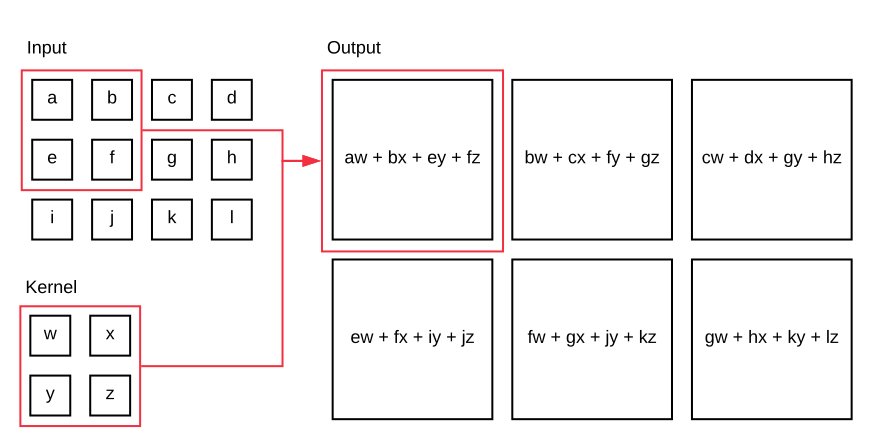
\includegraphics[width=\textwidth]{obrazky-figures/convolution.pdf}
    \caption{Convolution operation with 2D input data and 2D kernel}\label{fig:convolution}
\end{figure}

\subsection{Use of convolution in neural networks}

In machine learning, we leverage multiple important properties of the convolution operation:

\begin{itemize}
    \item Sparse interaction
    \item Sharing of parameters
    \item Equivariant representation
    \item Input of variable size
\end{itemize}

\subsubsection{Sparse interaction}

As you can notice in figure\,\ref{fig:convolution}, kernel can be of different size than input. When the input data is for example an image of millions of pixels, the size of kernel allows convolution to select only specific subset of inputs for each output. In traditional neural networks matrix multiplication is used instead of convolution. That means every output unit interacts with every input unit. In convolutional networks, the kernel size limits that just to certain subset of input units. It is called \textbf{sparse interaction}\,\cite[p.~335]{deeplearningbook} or \textbf{sparse weights} and it is accomplished by restricting kernel to a smaller size than the input. That results in smaller memory footprint of the model, since it requires fewer parameters to be stored. while at the same time it improves statistical efficiency. It has also impact on performance, since computing the output requires fewer operations compared to matrix multiplication. A graphical demonstration can be seen on figure\,\ref{fig:sparse_b}.

\begin{figure}[ht]
    \centering
    \includegraphics[width=.6\textwidth]{obrazky-figures/sparse_b.pdf}
    \caption{\textit{Sparse interaction viewed from below}: The highlighted units demonstrates propagation of one input unit from current layer $s_3$ to the next layer. On the top you can see all the output $n$ units, which are affected by this particular input. On the bottom image, you can see how the same situation is represented in traditional matrix multiplication.}\label{fig:sparse_b}
\end{figure}

Deep convolutional networks allow indirect interaction between units which would be out of reach for given kernel size. This property is called \textbf{receptive field}\,\cite[p.~337]{deeplearningbook} of a unit and can be seen when we look at the network from perspective of the output layer (see figure\,\ref{fig:sparse_a}).

\begin{figure}[ht]
    \centering
    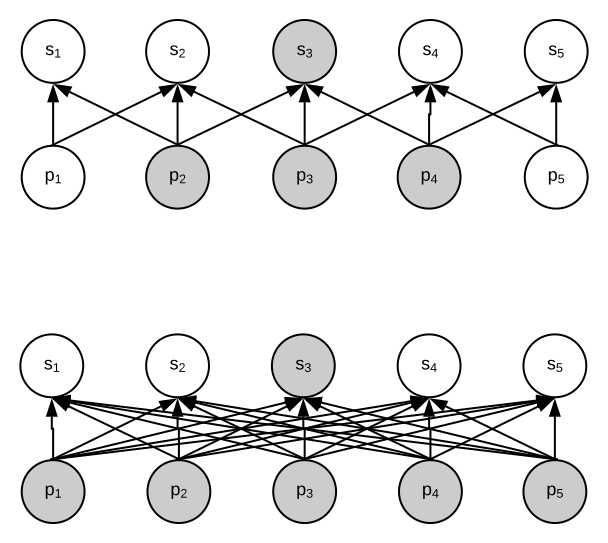
\includegraphics[width=.6\textwidth]{obrazky-figures/sparse_a.pdf}
    \caption{\textit{Sparse interaction viewed from above}: Highlighted portion of the image shows all units affecting current layer. The amount of units is smaller on the top picture. That represents sparse interaction. On the bottom is the same situation, when the current layer is formed by matrix multiplication in a traditional network.}\label{fig:sparse_a}
\end{figure}

However, this view limits us just to direct influence on a unit. Receptive field lists also indirect influence, hence when multiple convolutional layers are used by the network the field grows. The effect can be enhanced when network contains additional features like strided convolution or pooling. This means though the direct influence is very sparse, the final impact through indirect influence can make the units deeper in the network connected to most of the image on input.

\begin{figure}[ht]
    \centering
    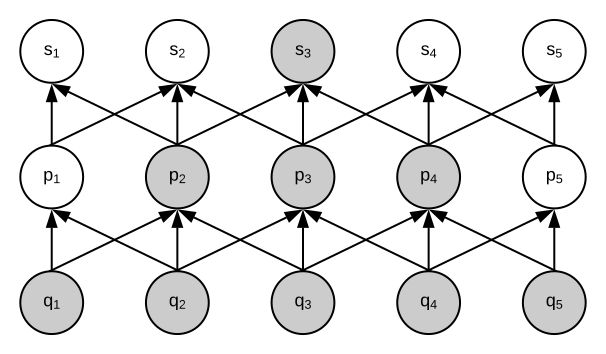
\includegraphics[width=.6\textwidth]{obrazky-figures/receptive.pdf}
    \caption{Receptive field}\label{fig:receptive}
\end{figure}

\subsubsection{Parameter sharing}

A feature of convolution referring to a reuse of of parameter in more than one computation. In matrix multiplication, each weight element is calculated and used only once when computing the output. The weight is multiplied by one element of the input and then never used again. In contrast, convolution keeps it's kernel the same an uses its elements for every output calculation. This brings an advantage of learning just one set of weights for the whole input, rather than computing and remembering a set of weights for each output unit. Parameter sharing has no impact on on forward propagation but it does further improve memory efficiency of a stored model.

\subsubsection{Equivariant representation}

A function is equivariant to another when $f(g(x)) = g(f(x))$. Convolution is naturally equivariant for example to translation\,\cite[p.~339]{deeplearningbook} . Imagine we have an input image and we shift the image some pixels to any direction. When convolution is performed, the same kernel is applied to any set of pixels, therefore the feature the network layer aims to collect can be found in the shifted image as well as in the original. It would just appear shifted in the output feature map. Here we can benefit from parameter sharing in use cases like edge detection. We're interested in the same feature, no matter where it appears on the image. In other use cases, like for example face detection, we might not be interested in the full parameter sharing. Imagine we have a kernel which is trained to detect mouth. In order to work properly, we should restrict this kernel to look for the feature only in bottom portion of the picture, because detecting a mouth on forehead would not result in proper outputs. We'll cover more about multi-kernel convolution layers later.

\subsubsection{Variable size of the input}

Convolution can process data samples of different sizes. When the use case requires to the network to be robust enough to properly process for example images, where each of the sample has different dimensions, this is a problem in matrix multiplication. The network can't apply the fixed size weight matrix on an input of different size. On the other hand, convolution is easy to perform, the situation is really similar to input of a fixed size, just the kernel is applied different amount of times.

\subsection{Pooling}

In neural networks, convolution layer doesn't mean solely convolution is applied. Typically such layer consists of multiple stages:

\begin{enumerate}
    \item \textbf{Convolution stage}: Multiple parallel convolutions are computed which produces a set of linear activations.
    \item \textbf{Detector stage}: Each of the linear activations from previous stage is run through a nonlinear activation function.
    \item \textbf{Pooling stage}: Further modification of the layer.
\end{enumerate}

The last, pooling stage, provides better understanding of the convolution output. Instead of returning a set of features, it reduces redundancy of neighbouring outputs and provides a summary statistics. This helps the network to be invariant small transition of the input. This means that if we translate the input of small amount of pixels, the outputs stay the same. This makes such network more robust. In a situations like a face detection, we don't need to know exact pixel coordinates of a feature, eye for example. We just need to define an are where we're looking for such feature.

There are many pooling operations, let's list some of the most popular ones like \textbf{max pooling}\,\cite{maxpooling} (reports the maximum output in rectangular neighbourhood), average of rectangular neighbourhood, $L^2$ norm of the rectangular neighbourhood, and weighted average of distance from the central pixel.

Invariance of transition is produced by pooling over spatial regions, though pooling layer can learn an invariance to a transformation of other kinds as well. That happens if we pool over outputs of other separately parametrized convolutions. As an example you can see an invariance to slant in cursive on figure\,\ref{fig:pooling}. This principle is accented mainly in maxout networks\,\cite{maxout}.

\begin{figure}[h]
    \centering
    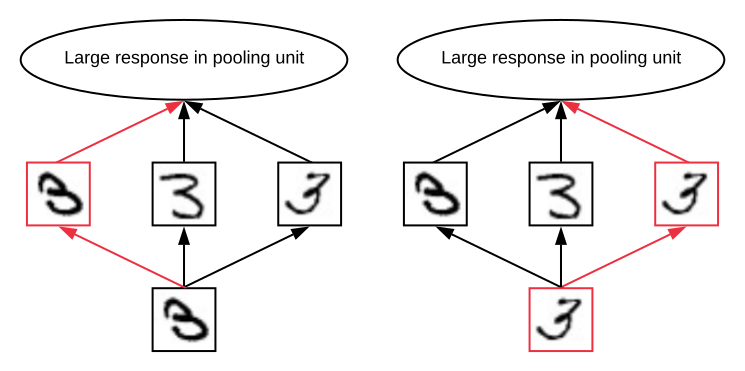
\includegraphics[width=.8\textwidth]{obrazky-figures/pooling.pdf}
    \caption{\textit{Pooling response with learned invariance to slant}: Here we have 3 filters, where all of them had a task to learn a handwritten number 3. Each of them resulted in learning of different slant of the number. When a number 3 is given as the input, one of the filters will match it and cause a high activation in corresponding detector unit. Due to use of pooling, the max pooling unit has a large activation as well, no matter which filter matched the number.}\label{fig:pooling}
\end{figure}

Since pooling can summarise a response of layer over whole neighbourhood of input units, it's not necessary to have the same amount of pooling units as the detector ones. We can leverage pooling to provide downsampling as can be seen in figure\,\ref{fig:downsample}. That further improves performance of the network since it lowers the amount of inputs for the next layer.

\textbf{Pooling with downsampling} is essential step when dealing with input of variable size. Let's say we want to use the convolution to detect a face on images with different resolution. We've learned our detectors to register mouth in the bottom half of the image and another two sets of detectors to locate eyes, each in one of the top quarters. We can use convolution layer with downsampling pooling to provide the required classification. We expect to be provided by 3 activations on the output, and each of the detector has assigned it's portion of the input. It doesn't matter if the portion contains this amount of pixels or much more.

\begin{figure}[h]
    \centering
    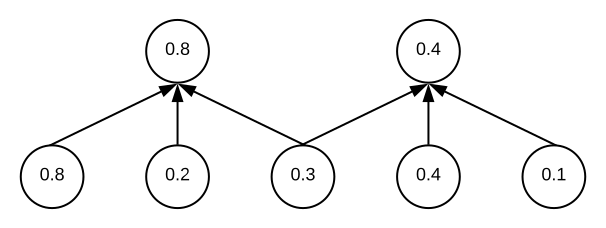
\includegraphics[width=.6\textwidth]{obrazky-figures/downsampling.pdf}
    \caption{Pooling with downsampling}\label{fig:downsample}
\end{figure}

In deep learning this is often the case. We don't refer to convolution as a simple single operation as described in the beginning of this chapter. Such convolution layer with single kernel would be capable of extraction only single feature, although in many spatial locations. Usually many convolutions are applied and performed in parallel. That can provide many different kernels for different features which are interesting for the use case. As a result network can locate many kinds of features at many locations.

\subsection{Strided convolution}

Also when we're already mentioning the downsampling in pooling, this step can be sometimes ommited and simplified even more. Although the result is similar to the pooling with downsample, the logic in based on different assumptions. In pooling we leverage all the information retrieved by the convolutions and simplify the output.

A strided convolution is rather avoiding some of the convolutions at all. That further lowers the computational costs, hence at a risk of not extracting all the features in such detail. In this case we sample pixels in every direction with a step $s$. This $s$ is called a \textbf{stride}. It's also possible to define a separate stride for each step direction.

\begin{figure}
    \centering
    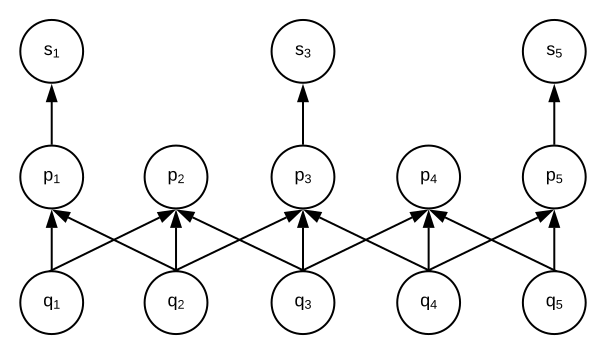
\includegraphics[width=.6\textwidth]{obrazky-figures/conv_down.pdf}
    \caption{Convolution and pooling with downsampling}\label{fig:conv_down}
\end{figure}


\begin{figure}
    \centering
    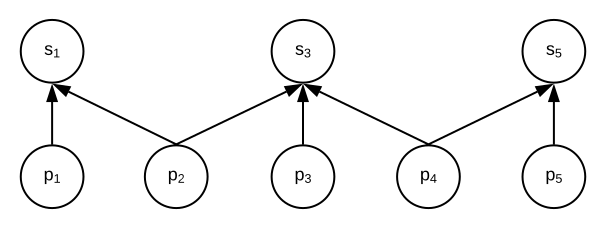
\includegraphics[width=.6\textwidth]{obrazky-figures/strided.pdf}
    \caption{Strided convolution}\label{fig:strided}
\end{figure}

As it can be clearly seen on the images\,\ref{fig:conv_down} and\,\ref{fig:strided} the two step downsampling is computationally more expensive than the strided optimisation.

\subsection{Zero padding}

Another feature which is essential to CNNs implementation is padding with zeros. This maintains the network's ability to preserve the width of its input if needed. The input tensor is padded with zeros on the ends, so a convolution operation doesn't shrink the size of input vector by a fraction of kernel. Without padding we are forced to either keep kernels small, or let the networks shrink in spatial extent. Both are extreme limitations of network's power. Padding allows to control independently both the size of kernel and resolution of the output.

\subsection{Other convolution layer types}

Sometimes our desire is to rather use locally connected layers. This resembles a discrete convolution with small kernel, but without parameter sharing. Therefore this layer type is sometimes called \textbf{unshared convolution}\,\cite{locally_connected}. Unshared type of convolutional layer is useful when we aim to detect features which are local and there's no assumption that the same feature should occur across all the input.

Another type available is \textbf{tiled convolution}\,\cite{tiled_conv} layer. A layer type meant to offer compromise between locally connected layers and convolutional layers. Instead of learning a set of weights for every spatial location, this layer type provides tiling. That means a single set of weights is learned and it is later applied in rotation, providing different set of weighs for neighboring locations. This makes the outcome similar to locally connected layer, while keeping a benefit of lower cost of convolutional layer, since requirements to store parameters would grow by factor of kernel set size, instead of size of whole feature map. A comparison overview of different convolution layer types can be seen on figure\,\ref{fig:compare_layers}

\begin{figure}
    \centering
    \includegraphics[width=.6\textwidth]{obrazky-figures/locally_connected.pdf} \\
    Locally connected \\
    \bigskip
    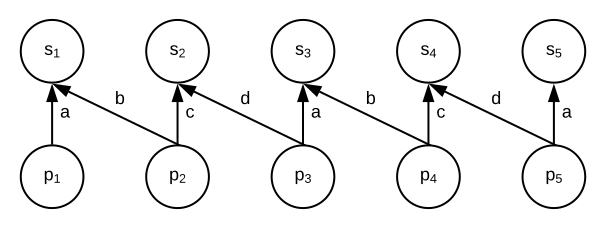
\includegraphics[width=.6\textwidth]{obrazky-figures/convolution_tiled.pdf} \\
    Tiled convolution \\
    \bigskip
    \includegraphics[width=.6\textwidth]{obrazky-figures/convolution_std.pdf} \\
    Standard convolution \\
    \bigskip
    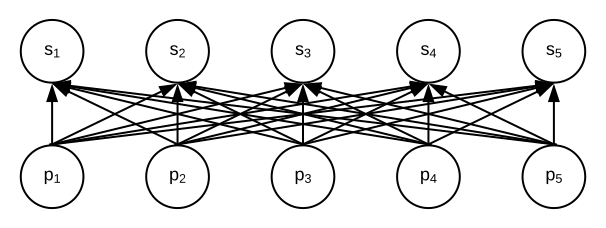
\includegraphics[width=.6\textwidth]{obrazky-figures/fully_connected.pdf} \\
    Fully connected \\
    \bigskip
    \caption{Comparison of convolutional layers}
    \label{fig:compare_layers}
\end{figure}

\section{Capsule neural networks}

Convolutional neural networks are a state-of-the-art of current deep learning. They are hugely popular and they can provide great results and solve problems which were unimaginable before. Despite all their power they embody fundamental drawbacks and limitations\,\cite{capsule_compare}. This and availability of grater computational power lead to creation of Capsule neural networks (CapsNET)\,\cite{capsule}.

\subsection{Rationale}

CNNs operate with features and their recognition. Deeper convolution layer detect
simple features, for example edges or color gradients. Layers higher in the network are designed to detect specific combinations of such features and creates more complex ones. And finally on the very top of the network a dense layer takes the very high level features and provide a prediction of a classification. And since many times the convolution is made invariant to different transformations, this can lead to impossible results. Mere presence of an object provides indication of feature presence. Relation between detected features is not considered at all. When simple features are composed to a more complex one, translational or rotational relationship doesn't play any role.

We've already tackled the way CNN is using to deal with this problem. Pooling and more convolutional layers of smaller kernels are applied to reduce spatial size of information lost during each convolution. This aims to increase the field of view for convolutional layers higher in the network, therefore allows them to locate features in larger portion of the input image. Pooling made CNNs surprisingly effective and top performing architecture so far, though still enhancing loss of information.

Prof. Geoffrey Hinton, one of fathers of deep learning and author of many architectures and algorithms is also the author of capsule neural networks. Hinton wrote\,\footnote{\url{https://www.reddit.com/r/MachineLearning/comments/2lmo0l/ama_geoffrey_hinton/clyj4jv/}}:
\begin{quotation}
    The pooling operation used in convolutional neural networks is a big mistake and the fact that it works so well is a disaster.
\end{quotation}

To demonstrate this drawback imagine a CNN face detector. Deeper layers of network detects parts of facial features. The higher layers combines these parts into complex features like an \textit{eye}, \textit{nose} or \textit{mouth}. Our multi-kernel convolution would allow us to define regions where we expect such features, though we can't define the relation between them. The network can simply recognise an image as a valid face, despite for example the \textit{eye} is rotated to the opposite direction than a \textit{mouth}. A demonstration of such problem can be seen on figure\,\ref{fig:capsule_face}.

\begin{figure}[h]
    \centering
    \includegraphics[height=0.3\textwidth]{obrazky-figures/face_normal.pdf}
    \hspace{10em}
    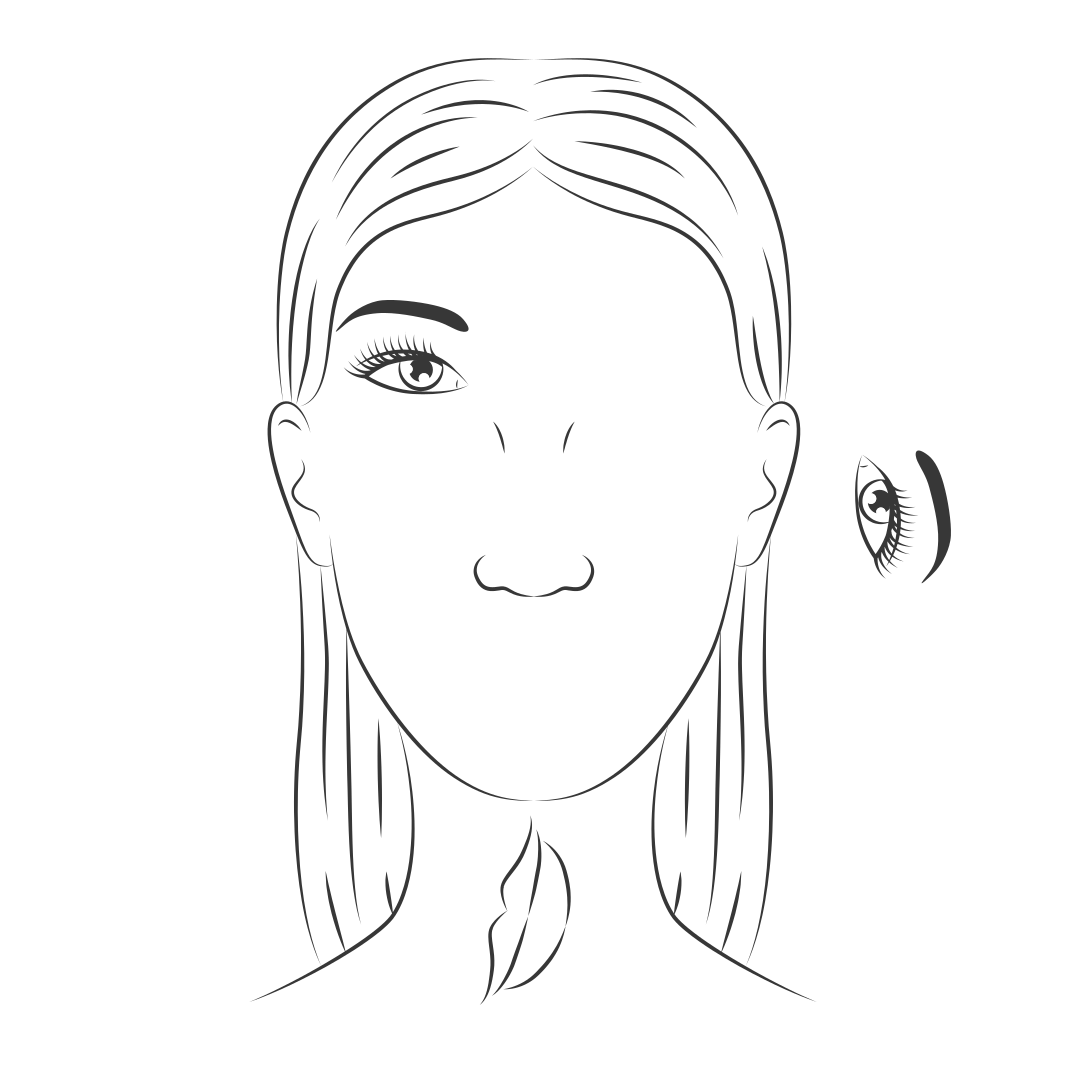
\includegraphics[height=0.3\textwidth]{obrazky-figures/face_disorted.pdf}
    \caption{Both of these images can be evaluated to be a face. Spatial location, relation and pose between simpler features are not considered by this type of network. Both images appear similar to CNN. \textit{Original artwork provided by Freepik\,\cite{freepik}}}
    \label{fig:capsule_face}
\end{figure}

\subsection{Inverse graphics}

Hinton, inspired by computer graphics, tried to explain and reconstruct human brain's visual cognitive functions. The brain itself in fact does the opposite process to \textit{rendering}. Hinton calls it \textbf{inverse graphics}. A visual information is decomposed into a hierarchical representation of objects, which are matched against known, learned patterns. This relationship matrix is stored in our brains. One key factor is that object representation is not dependent on view angle.

So how do we model this hierarchical relationship inside a neural network? Here we can learn from solutions already discovered in another field -- in computer graphics. 3D modeling uses something called a \textbf{pose}. This represents relation between 3D objects and provides a rotation and translation transformation matrix. In neural networks we represent that as a 4D \textit{pose matrix}\,\cite{capsule}. This results in combination of information about object relations with internal representation of object data. Hence it becomes easy for a model to recognise that it just sees a different view of something it already saw before.

\begin{figure}[h]
    \centering
    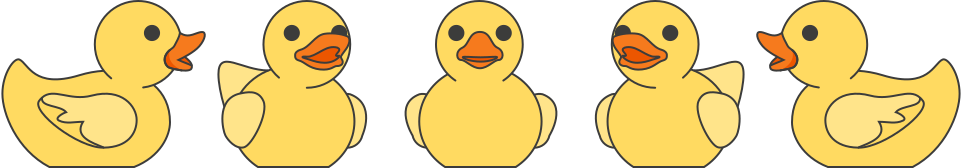
\includegraphics[width=.8\textwidth]{obrazky-figures/duck.pdf}
    \caption{CNN struggles to recognise this is the same object. Human brain, on the other hand, immediately understands that objects on the picture are identical, despite being viewed from multiple different angles. \textit{Original artwork provided by Freepik\,\cite{freepik}}}
    \label{fig:duck}
\end{figure}

Let's discuss situation on the figure\,\ref{fig:duck}. A human looking at this picture can easily recognise, it is a rubber duck viewed from different angles. Our internal representation of rubber duck is independent on the viewing angle. It may be the first time that these particular pictures are shown to you, although you simply know their meaning. Since there's no internal representation of 3D space in CNNs, it really struggles. On the other hand, for CapsNET, this problem is pretty easy since the 3D relations are explicitly modeled. Experiments shown that usage of capsule neural networks can reduce error rate from $20\%$ to $12\%$\,\cite{capsule_compare}.

And this is not the only benefit of usage of capsules. It also significantly lowers the amount of data required to train such network to achieve comparable performance to a CNN. And this make sense, since capsule theory is much closer to the way how brain does work. If a brain tries to learn to distinguish a horse from a cow, it only needs to be presented with few images, at most couple of dozens. CNN would require to be presented by many thousands of image samples, to achieve comparable performance. In this particular aspect we can compare CNNs to a brute-force approach to deep learning.


\chapter{Available solutions}
\label{chapter:solutions}
Before implementing own solution, let's firstly uncover some available and current solutions to this very problem. Naturally, big progress and research is performed in this topic, therefore this chapter is not meant to provide full market scan, or list every solution available. It rather aims to discover some fine examples of neural network implementations which perform well.

Later on you'll stumble upon a list of available face recognition databases and data sets which can be used for training and evaluating the very own implementation. Each of the data set description is accompanied by a short list of their respective metrics.

\section{Existing implementations}

\subsection{\dots}\todo{Add solutions}

\subsection{FaceNET}\todo{Desctibe facenet}


\section{Frameworks}

Each of the previously mentioned solutions has something in common. They've used a AI framework or library of some sort. Writing neural networks from scratch is obviously a complex task, therefore there are many initiatives which seeks to simplify and facilitate access to such complex structures. Let§s list some most common ones and list some of their basic advantages and disadvantages.

\subsection{Torch and PyTorch}

Torch is a deep-learning and computational framework written in Lua. While very powerful, its design prevented from being adopted by users and researchers. The main problem was in usage of rather exotic programming language which created barrier for users. It's been decided to create a Python clone of the framework, which brought PyTorch to existence. It was created by Facebook and released in 2007 under an open source license. One of it's key features are dynamic computation graphs, which can serve well when processing inputs or outputs of variable length.

\begin{itemize}
    \item[$\boldsymbol{+}$] Many pluggable modules
    \item[$\boldsymbol{+}$] Easy to integrate different extensions
    \item[$\boldsymbol{+}$] Simple to define own layers
    \item[$\boldsymbol{+}$] Straightforward access to running code on GPU
    \item[$\boldsymbol{+}$] Offers dynamic computation graphs
    \item[$\boldsymbol{+}$] Broad community and wide audience
    \item[$\boldsymbol{+}$] Easier to inspect and monitor training of models
    \item[$\boldsymbol{+}$] Intuitive API
    \item[$\boldsymbol{-}$] Requires custom training code
\end{itemize}

\subsection{Tesorflow}

This library created by Google was designed as a replacement for their previous project called Theano. Tensorflow a heavyweight framework written as a Python API in C/C++. It simplifies researcher's task in many ways better than other frameworks. For example it generates a computational graph and performs automatic differentiation. That means the user is not required to write a training code (backpropagation) every time, he's experimenting with a new network topology. Since this framework is backed by Google it thrives in many different applications and can scale across devices. Many posibilities for applying saved models in different environment enables use of AI in mobile devices and even in web browsers. However it's broad possibilities and options make this framework hard to understand and for newcomers it can be confusing and too complex. Therefore an abstraction layer above Tensorflow had been created, but more about that in the Keras subsection below.

\begin{itemize}
    \item[$\boldsymbol{+}$] Native Python and Numpy integration
    \item[$\boldsymbol{+}$] Automatic training code
    \item[$\boldsymbol{+}$] Broad community and wide audience
    \item[$\boldsymbol{-}$] Heavyweight frameworks
    \item[$\boldsymbol{-}$] A bit slower than PyTorch
\end{itemize}

\subsection{Caffe and Caffe2}

Caffe is another competition framework, which is widely popular among researchers. It started as a C/C++ port of Matlab's implementation of fast convolutional networks. It's mainly oriented on feed forward networks and image processing and is not intended for other deep learning application like text processing or 1D series data. Later on it became performace wise obsolete and community of Caffe developers decided to start from scratch and created a long-awaited successor Caffe2. Backed by Facebook as their second deep learning toolkit after PyTorch it provides more lightweight and scalable solution than before. It's main area of focus is enterprise grade production environments.

\begin{itemize}
    \item[$\boldsymbol{+}$] Great for image processing and feedforward networks
    \item[$\boldsymbol{+}$] Automatic training code
    \item[$\boldsymbol{+}$] Lightweight
    \item[$\boldsymbol{+}$] BSD license
\end{itemize}

\subsection{Keras}

A modern abstraction layer above Tensorflow. Authors and users of Tensorflow suffered from heavy and complex code structures and when PyTorch appeared with their light and straightforward Python API, they've started adopting the same principals for the Tensorflow as well. Therefore a project named Keras was created. It provides intuitive API inspired by Torch and while starting from Tensorflow it outgrown this base and spread across many deep learning libraries as its backeds - Theano, Deeplearning4j, and CNTK. In addition to its high level abstraction over the backends Keras also provides means to drill down and optimize and manipulate the underlying code.

\begin{itemize}
    \item[$\boldsymbol{+}$] Intuitive API
    \item[$\boldsymbol{+}$] Multiple backeds to choose from
    \item[$\boldsymbol{+}$] Lightweight
    \item[$\boldsymbol{+}$] Fask growing community
    \item[$\boldsymbol{+}$] Recognized as a standard Python API for neural networks
\end{itemize}

\section{Data Sets}

In order to better understand the nature of CCTV imagery, pictures in the wild and the source data we are about to work with, let's describe some commonly used databases of face images and face recognition data. It's crucial to understand the variety and differences between subjects captured on sample images, like their age, sex, and ethnicity. Also we need to pay attention to circumstances of the photo setup. That means for example consistency of resolution across samples, poses and angles, etc.

\subsection{FDDB: Face Detection Data Set and Benchmark}

This data set provides annotations for Faces in the Wild\,\cite{fiw} database. FDDB\,\cite{fddb} lists coordinates for bounding boxes of over 5 thousands faces located on pictures from Faces in the Wild database. Usually multiple faces are located on a single picture. This data set can provide ground for face detection algorithm and therefore it can be benefited from in the first step of implementation. For recognition of individuals whom such face belongs to, another data set has to be used. A great accompanying data set can be the LFW mentioned in next subsection.

\begin{table}[ht]
    \centering
    \caption{FDDB data set metrics}

    \begin{tabularx}{0.75\textwidth}{l|l}
        \toprule
        Number of subjects & \num{5171} \\
        Total images &  \num{28045} \\
        Poses & Varies \\
        Resolution & All kind, even blurred faces \\
        \bottomrule
    \end{tabularx}
\end{table}

\subsection{LFW: Labeled Faces in the Wild}

LFW\,\cite{lfw} provides labels for images from Faces in the Wild data set mentioned before. Therefore when used in conjunction with FDDB\dots\todo{LFW in more detail}

\begin{table}[ht]
    \centering
    \caption{LWF data set metrics}

    \begin{tabularx}{0.75\textwidth}{l|l}
        \toprule
        Number of subjects &  \\
        Total images &  \\
        Samples per subject &  \\
        Resolution &  \\
        License &  \\
        \bottomrule
    \end{tabularx}
\end{table}

\subsection{The Extended Yale Face Database B}

Extended version of original Yale Face Database. The extension was provided by UCSD\,\cite{ext_yale_paper}. This database comprises over \num{16000} images of 28 unique subjects. They are fitted to same size and resolution, covering various angles of the face. There are 9 poses provided for each person, each of them covering 64 different illumination condition.  When compared to a large scale data set this database lacks volume, however it maintains consistency across its samples.

\begin{table}[ht]
    \centering
    \caption{Extended Yale Face Database B metrics}

    \begin{tabularx}{0.75\textwidth}{l|l}
        \toprule
        Number of subjects & 28 \\
        Total images & \num{16128} \\
        Samples per subject & 576 \\
        Poses & 9 \\
        Resolution & 168x192 pixels \\
        License & Free to use for research purposes\\
        \bottomrule
    \end{tabularx}
\end{table}

\subsection{SCface - Surveillance Cameras Face Database}

A face database originate from University of Zagreb. Quaility data set of surveillance like face images. It aims to simulate a CCTV captured images by simulating an uncontrolled indoor environment. Each of 130 subjects is captured by up to 8 video survailence cameras. Some of them even capable of IR capturing. Each camera produces images of different resolution and sharpness. Cameras are also set in different angles against the subject. SCFace\,\cite{scface} mimics real-world circumstances and use cases of CCTV, therefore this data set can be used to train robust solutions for face recoginition targeting CCTV and survailence cameras.

A disadvantage is the size of this data set, where we can find \num{4160} image samples only. When compared to large-scaled data set like the VGGFace and VGGFace2 mentioned in next subsection, this data set lacks volume. Also the variety of subjects is not robust enough in comparison to other data set. As said, SCFace captures 130 subjects. Most of them are of the same sex, all of the same ethnicity.

\begin{table}[ht]
    \centering
    \caption{SCFace data set metrics}

    \begin{tabularx}{0.75\textwidth}{l|l}
        \toprule
        Number of subjects & 130 \\
        Total images & \num{4160} \\
        Samples per subject & Fixed amount of 32 images per person \\
        Resolution & Varies, 3 different sizes \\
        License & Custom \\
        \bottomrule
    \end{tabularx}
\end{table}

This database is available for research purposes and upon written request to the authors.

\subsection{VGGFace2}

Visual Geometry Group produced a second iteration of their face recognition data set\,\cite{VVGFace2}. This is one of the most wide data sets which are publicly available. It provides a wide-scale data for face recognition for over 9000 different identities. Distribution of individuals varies though, with minimal 87 images up to 843 per identity. Average number of images per subject is 362. The data set contains over \num{3.3} milion of images. Subjects varies in ethnicity, age and profession, while the images varies in angles or poses.

The data set is made available under Creative Commons license\,\cite{cc_by-sa_40}, therefore it's available for broad use to any project.

This project also provides sample models trained on this data set. However, the example pretrained neural network models provided within this project are not the sole example of the data set usage. Many popular face recognition models are trained on this data set. For example FaceNET can be seen as one of the popular projects which benefits from this data set.

\begin{table}[ht]
    \centering
    \caption{VGGFace2 data set metrics}

    \begin{tabularx}{0.75\textwidth}{l|l}
        \toprule
        Number of subjects & \num{9294} \\
        Total images & \num{3311286} \\
        Samples per subject & Varies, 87--843 per subject \\
        Resolution & Varies, many different sizes \\
        License & Creative Commons\,\cite{cc_by-sa_40} \\
        \bottomrule
    \end{tabularx}
\end{table}


% \chapter{Discussion}
% \label{chapter:discussion}

\chapter{Conclusion}
\label{chapter:conclusion}
\listoftodos

%=========================================================================


  % Kompilace po částech (viz výše, nutno odkomentovat)
  % Compilation piecewise (see above, it is necessary to uncomment it)
  %\subfile{projekt-01-uvod-introduction}
  % ...
  %\subfile{chapters/projekt-05-conclusion}


  % Pouzita literatura / Bibliography
  % ----------------------------------------------
\ifslovak
  \makeatletter
  \def\@openbib@code{\addcontentsline{toc}{chapter}{Literatúra}}
  \makeatother
  \bibliographystyle{bib-styles/slovakiso}
\else
  \ifczech
    \makeatletter
    \def\@openbib@code{\addcontentsline{toc}{chapter}{Literatura}}
    \makeatother
    \bibliographystyle{bib-styles/czechiso}
  \else
    \makeatletter
    \def\@openbib@code{\addcontentsline{toc}{chapter}{Bibliography}}
    \makeatother
    \bibliographystyle{bib-styles/englishiso}
  %  \bibliographystyle{alpha}
  \fi
\fi
  \begin{flushleft}
  \bibliography{project-20-bibliography}
  \end{flushleft}

  % vynechani stranky v oboustrannem rezimu
  % Skip the page in the two-sided mode
  \iftwoside
    \cleardoublepage
  \fi

  % Prilohy / Appendices
  % ---------------------------------------------
  \appendix
\ifczech
  \renewcommand{\appendixpagename}{Přílohy}
  \renewcommand{\appendixtocname}{Přílohy}
  \renewcommand{\appendixname}{Příloha}
\fi
\ifslovak
  \renewcommand{\appendixpagename}{Prílohy}
  \renewcommand{\appendixtocname}{Prílohy}
  \renewcommand{\appendixname}{Príloha}
\fi
%  \appendixpage

% vynechani stranky v oboustrannem rezimu
% Skip the page in the two-sided mode
%\iftwoside
%  \cleardoublepage
%\fi

\ifslovak
%  \section*{Zoznam príloh}
%  \addcontentsline{toc}{section}{Zoznam príloh}
\else
  \ifczech
%    \section*{Seznam příloh}
%    \addcontentsline{toc}{section}{Seznam příloh}
  \else
%    \section*{List of Appendices}
%    \addcontentsline{toc}{section}{List of Appendices}
  \fi
\fi
  \startcontents[chapters]
  \setlength{\parskip}{0pt}
  % seznam příloh / list of appendices
  % \printcontents[chapters]{l}{0}{\setcounter{tocdepth}{2}}

  \ifODSAZ
    \setlength{\parskip}{0.5\bigskipamount}
  \else
    \setlength{\parskip}{0pt}
  \fi

  % vynechani stranky v oboustrannem rezimu
  \iftwoside
    \cleardoublepage
  \fi

  % Přílohy / Appendices
  \chapter{CD Content}

\begin{itemize}
    \item \texttt{src}: Source codes for \texttt{CapsNet} package.
    \item \texttt{src/notebooks}: Example \textit{Jupyter} notebooks for training and testing a model.
    \item \texttt{src/saved\_models}: Saved models ready to be imported and used.
    \item \texttt{src/README.md}: Installation and usage manual.
    \item \texttt{thesis}: Source codes to build this thesis PDF.
    \item \texttt{thesis.pdf}: This very same thesis as a PDF file.
\end{itemize}


  % Kompilace po částech (viz výše, nutno odkomentovat)
  % Compilation piecewise (see above, it is necessary to uncomment it)
  %\subfile{projekt-30-prilohy-appendices}

\end{document}
